\subsubsubsubsection{House}
\begin{figure}[h]
\centering
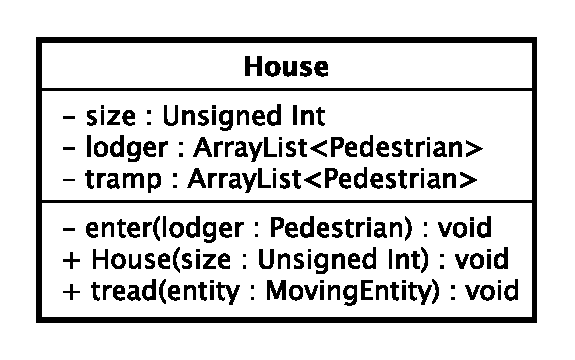
\includegraphics[scale=0.6,keepaspectratio]{images/solution/house.eps}
\caption{App::Reactive::House}
\label{fig:sd-app-house}
\end{figure}
\FloatBarrier
\begin{itemize}
  \item \textbf{Description} \\
    It represents a house which can host several pedestrians.
  \item \textbf{Attribute}
  \begin{itemize}
    \item \texttt{- size: Unsigned Int} \\
The maximum number of pedestrians that can be hosted into the house.
    \item \texttt{- lodger: ArrayList<Pedestrian>} \\
The list of pedestrian that are currently hosted into the house.
    \item \texttt{- tramp: ArrayList<Pedestrian>} \\
The list of pedestrian that are currently outside the house, waiting to enter into the house.
  \end{itemize}
  \item \textbf{Operation}
  \begin{itemize} 
    \item \texttt{- enter(lodger: Pedestrian)} \\
The house is not full and the pedestrian become a lodger.   
    \item \texttt{+ House(size: Unsigned Int)} \\
Creates a house specifying its maximum number of lodgers.
\item \texttt{+ tread(entity: MovingEntity)} \\
Implements the permanence of the pedestrian into the house. First the house notifies the moving entity that there is a building in the current stretch. After receiving a reply, the house checks the the entities specified in the reply message and puts them in the right queue: if the house is not full it invokes enter, otherwise the pedestrian is placed in the tramp queue. At the end the house register itself for a timeout notification.
  \end{itemize}
\end{itemize}
